\section{Implementation and computational illustration}\label{sec:computation}

The experiments in this section test whether the predicted grid sizes appear
in practice and whether the certificates are cheap enough to check. They are
not a benchmark of competitive performance: the implementation is a reference
code in exact rational arithmetic, and most instance families are small and
designed.

\subsection{Implementation}\label{sec:comp-impl}
The reference implementation is written in Python with exact rational
arithmetic (Python's \texttt{fractions} module); floating-point input is
rejected. It handles explicit box QPs $\frac12x^\T Hx+b^\T x+c$ with continuous
and integer coordinates, supplied or heuristically computed (minimum-fill)
tree decompositions with arbitrary branching, and empty separators. It
implements the corrected grids of Section~\ref{sec:grids} with corrections
$\max\{H_{ii},0\}w^2/8$, the two-node grids $\{\ell_i,u_i\}$ for coordinates
with $H_{ii}\le0$, two-pass dynamic programming with all min-marginals,
filtering, and CT (Algorithm~\ref{alg:ct}) in the common-mesh form of
Lemma~\ref{lem:commonmesh}. It differs from the analysis in the following
ways.
\begin{enumerate}[label=(\alph*)]
\item All coordinates share the mesh $h_j=s2^{-j}$, and the analysis that
applies is Lemma~\ref{lem:commonmesh} with the Euclidean condition number
$\kappa$, not Theorem~\ref{thm:approx}.
\item The cap of trial $\mu$ is $100\cdot2^\mu\lceil\log_2(n+2)\rceil$,
$12.5$ times the cap of Lemma~\ref{lem:commonmesh}, and the stage limit is the
least $J$ with $\frac78Lns^24^{-J}\le\varepsilon$ instead of
$\frac9{16}Lns^24^{-J}\le\varepsilon$, so a trial may run one stage longer.
\item Each trial starts with the center at the current incumbent instead
of~$\ell$. Validity and the rate analysis allow any first center (the bound
on $\norm{c-x^*}$ in (G2) of Lemma~\ref{lem:commonmesh} holds at $j=0$ for
every $c\in X$); the bit-length analysis of Appendix~\ref{app:growth} does
not cover it.
\item Before stage~$0$, two sweeps of exact coordinate descent from $\ell$,
$u$ and the box midpoint provide the first incumbent; after each stage the
same descent, within the current box, starts from the grid minimizer $y_j$.
An optional presolve certifies convex instances by an exact $LDL^\T$ factorization and a rational
KKT point.
\item The reported lower bound is the largest bound of all stages and trials,
including the initial interval bound, rather than $\beta_j$ of the last
stage.
\item The ``uniform'' grids of the experiments below are the grids of
Definition~\ref{def:graded} with $\theta=0$ around one center, not the unions
of cells of UC (Algorithm~\ref{alg:uc}).
\item The exact-output wrapper, which implements EX (Algorithm~\ref{alg:ex}),
uses the acceptance rule of Proposition~\ref{prop:accept} with the row-sum
height constant of Remark~\ref{rem:heights}, with a common denominator that
also clears $H_{ij}/2$; this constant is never smaller than the one
in~\eqref{eq:exact-constants}. It starts at $q=4$, doubles $q$ after each
round, restarts the grid solver from the full box in every round with the
incumbent as its first center, and tests three candidates after each round:
the incumbent, its coordinatewise rational reconstruction
(Remark~\ref{rem:cf}) and the stationary point of REC
(Algorithm~\ref{alg:rec}).
\end{enumerate}
None of these affects validity. Experiments E1--E3 below run single trials,
that is, TRIAL (Algorithm~\ref{alg:trial}) with the common mesh, a fixed
grading~$\theta$ ($\theta=0$ for uniform grids), no cap on the nodes per
coordinate and a fixed number of stages, in E1 also without filtering; the
``theorem'' grading is the largest $2^{-\mu}$ with $8\kappa\theta^2\le1$ for the certified upper bound on
$\kappa$, which the algorithm itself does not know. The default schedule of
E2, the comparison with SCIP (E5), the random family E6, experiment S1, the
chain and the recourse runs use CT. In E2, E5, E6 and the chain no trial was
aborted by the cap: the only restarts occurred in E2, and each followed a
trial that reached its stage limit.

Certificates store the grids, the directed messages and the filtering
decisions of every stage, which is more than Theorem~\ref{thm:certificate}
requires. A separate checker recomputes every table and message, checks the
Bellman equalities, the min-marginals, every exclusion, the incumbent values
and the final status, and never calls the grid generator, the dynamic program
or the filtering code of the solver; it shares model parsing, decomposition
validation and objective evaluation with the solver. The checker is
independently written, not formally verified. On the runs of E1--E6, the
chain and the plain-grid recourse runs below with a solve time of at least
$0.1$ seconds, replay took between $0.81$ and $2.54$ times as long as the
solve. Further modules implement exact linear and convex
box-QP oracles with
primal, dual or Farkas witnesses, affine recourse recognition and lifting,
minimum-cut and convex value-factor recourse, the TU-constrained grids, the
endpoint optimal-set descriptor and explicit polynomial factors, each with its
own checker; the convex value-factor and recourse checkers reuse the solver's
grid, table and lifting code, so only the main checker is independent in the
sense above. Code, inputs, raw results and reproduction scripts (one command
per experiment group) accompany the paper.

All runs below used one thread per process and at most four processes on an
Intel Xeon w5-2565X under Windows Subsystem for Linux (WSL2) with
Python~3.13, on a machine shared with unrelated long-running jobs (load average 11 to 19). Timings are single
measurements and indicative only. Every certificate on which a result in
Sections~\ref{sec:comp-growth}--\ref{sec:comp-recourse} rests was replayed by
its checker, and every replay was valid; the runs of S1 that only count
stages (Section~\ref{sec:comp-localized}) were not replayed.

\subsection{Accuracy independence, conditioning and dimension}
\label{sec:comp-growth}
The planted family consists of nonconvex quadratics on $[-1,1]^n$ with Hessian
$H=2I+C$, where $C$ has path, random-tree or band sparsity. About a quarter of
the coordinates are at a bound at the planted minimizer $x^*$, all with a
strictly inward derivative of the same size; the other coordinates of $x^*$
are of the form $k/21$ with $\abs k\le10$, and on them the Hessian block
$H_{J_0J_0}$ has smallest eigenvalue $4/\kappa_{\mathrm{target}}$, up to a
rounding of the coupling scale to a multiple of $2^{-12}$. Entries of $C$ that
touch an active coordinate have size $2$ to $4$, and $H$ is indefinite in
every instance (its smallest eigenvalue is at most $-1.75$).
Lemma~\ref{lem:growthcert}(a) gives the certified lower bound $g_0$ on the
growth constant, by an exact $LDL^\T$ test of $H+2M-2g_0I$, and part~(b) with
a rational approximate eigenvector of $H_{J_0J_0}$ gives an upper bound;
with $L=2$ this brackets $\kappa$ to within $12\%$. The family is benign in
one respect: once $x^*$ is known, \eqref{eq:minorant} certifies it directly;
the grid solver does not use this.

The minimizers are mostly off the grids. Within a trial every node of
coordinate $i$ is either a dyadic rational or the sum of the first center
$c_i^{(0)}$ and a dyadic rational, because the endpoints $\pm1$, the meshes
and the gradings are dyadic, filtering moves endpoints only to nodes, and every
later center is a node. A coordinate $x^*_i=k/21$ with $k\ne0$ is therefore a
node only if $c_i^{(0)}$, which the coordinate descent provides, differs from
$x^*_i$ by a dyadic rational. Over the runs of E1--E3 with
$\kappa_{\mathrm{target}}\ge4$, 347 of 3{,}177 free coordinates of $x^*$,
counted once per run ($11\%$), were nodes of the last grid. Of the 153 such
coordinates in the 78 single-trial runs of E1 with filtering and of E3, 146 had
already been set to $x^*_i$ by the initial descent, 3 had $x^*_i=0$, and in the
other 4 the first center differed from $x^*_i$ by a nonzero dyadic rational.

\begin{figure}[t]
\centering
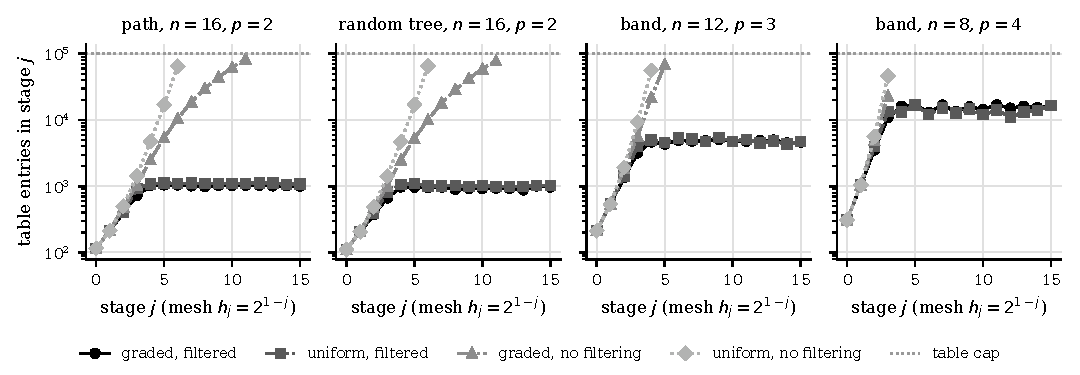
\includegraphics[width=\textwidth]{figures/E1_states_vs_stage.pdf}
\caption{Experiment E1: table entries per stage against the stage index $j$
(mesh $h_j=2^{1-j}$), median of three seeds, for graded and uniform grids with
and without filtering; $\theta=1/8$, $\kappa\in[3.99,4.45]$. A stage is plotted
only if all three runs completed it. Runs without filtering stop at the cap
of $10^5$ table entries per stage (dotted line).}\label{fig:E1}
\end{figure}

\paragraph{E1: accuracy.} Figure~\ref{fig:E1} shows the effect of filtering in
single trials with $\theta=1/8$. On the path with $n=16$, filtered graded
grids use about $1{,}000$ table entries per stage from stage~4 to stage~15,
while unfiltered graded grids reach $83{,}161$ entries at stage~11 and
unfiltered uniform grids $64{,}879$ at stage~6, after which both hit the cap.
Filtered uniform grids also plateau (about $1{,}100$ entries): filtering, not
the grading, removes the dependence on the accuracy. This is predicted by
(G1)--(G4) of Lemma~\ref{lem:commonmesh}, which also hold for $\theta=0$, so
the retained radius is still at most $4.2\sqrt{n\kappa}\,h_j$ and the next
uniform grid has at most $16.8\sqrt{n\kappa}+3$ nodes per continuous
coordinate. In the graded runs of E1 with filtering and the runs of E2 and E3
with the theorem's grading, all of which satisfy $8\kappa\theta^2\le1$, the
measured quantities stayed far below the bounds of
Lemma~\ref{lem:commonmesh} at all 876 stages: the gap $D(y_j)$ was at most
$0.16\,Lnh_j^2$ (bound $\frac9{16}Lnh_j^2$), the retained radius at most
$0.18$ of $4.2\sqrt{n\kappa}\,h_j$, and the number of nodes per coordinate at
most $5\%$ of the cap $8\theta^{-1}\lceil\log_2(n+2)\rceil$ (and at most
$0.4\%$ of the implementation's cap). The radius ratio uses the lower end
of the certified interval for $\kappa$, which can only increase it.

\begin{figure}[t]
\centering
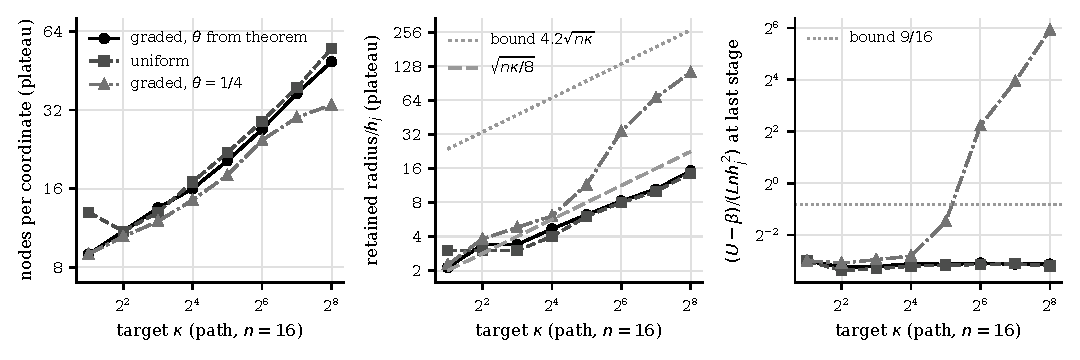
\includegraphics[width=\textwidth]{figures/E2_plateau_vs_kappa.pdf}
\caption{Experiment E2: path with $n=16$ and $\kappa_{\mathrm{target}}=
2,4,\dots,256$; the certified $\kappa$ lies in
$[0.97\,\kappa_{\mathrm{target}},1.12\,\kappa_{\mathrm{target}}]$. Left: nodes per
coordinate, the maximum over free coordinates and the median over the last
four stages and the three seeds. Middle: retained radius over $h_j$, same
statistics, with the bound $4.2\sqrt{n\kappa}$ of Lemma~\ref{lem:commonmesh}
and the reference $\sqrt{n\kappa/8}$, both evaluated at the lower end of the
certified $\kappa$ interval. Right: gap $U-\beta$ at the last stage over
$Lnh_j^2$, with the bound $9/16$; with the fixed grading $\theta=1/4$, which
violates $8\kappa\theta^2\le1$ for $\kappa_{\mathrm{target}}\ge4$, contraction
fails for $\kappa_{\mathrm{target}}\ge64$.}
\label{fig:E2}
\end{figure}

\paragraph{E2: conditioning.} Figure~\ref{fig:E2} varies $\kappa$ on the
path. With the theorem's grading the plateau grows from 9 to 49 nodes per
coordinate, and the retained radius grows somewhat more slowly than
$\sqrt\kappa$ and stays far below its bound. With the fixed grading
$\theta=1/4$ the condition $8\kappa\theta^2\le1$ fails for every instance with
$\kappa_{\mathrm{target}}\ge4$; the trial still contracted for
$\kappa_{\mathrm{target}}\le32$, but for $\kappa_{\mathrm{target}}\ge64$ the
last-stage gap divided by $Lnh_j^2$ was $4.7$, $15$ and $61$. CT handled this
automatically: it succeeded in its first trial ($\theta=1/4$) for
$\kappa_{\mathrm{target}}\le32$ and restarted once or twice for larger
$\kappa_{\mathrm{target}}$, earlier than Lemma~\ref{lem:commonmesh}
guarantees. For
$\kappa_{\mathrm{target}}=2$ the generator sets the couplings between free
coordinates to zero ($H_{J_0J_0}=2I$); the free coordinates are then
separable, and the initial coordinate descent already returns~$x^*$.

\paragraph{E3: dimension.} On paths with $n=4,8,\dots,128$ and
$\kappa_{\mathrm{target}}=4$ (coupled free coordinates,
$\kappa\in[3.99,4.45]$), filtered uniform grids grew from 7 to 26 nodes per
free coordinate, graded grids with the theorem's grading $\theta=1/8$ from 9
to 19, and graded grids with $\theta=1/4$ from 9 to 17. This range of $n$ is
too small to separate $\log n$ from $\sqrt n$ cleanly;
Corollary~\ref{cor:uniformgrid} shows that uniform grids need order
$\sqrt{n\kappa}$ nodes on some instances.
On the separable instances with $\kappa_{\mathrm{target}}=2$, filtered
uniform grids used exactly $4(\lfloor\sqrt{n/4}\rfloor+1)+1$ nodes; we report
the coupled case because the separable one does not test coupling.

\subsection{Random instances without planted structure}\label{sec:comp-random}
Experiment E6 uses unplanted random continuous box QPs on $[-1,1]^n$ with path
or band (bandwidth~2) sparsity, $n=8,12,16,24$ and five seeds each: diagonal
entries $k/2$ with $k$ uniform in $\{-4,\dots,8\}$, interaction entries $\pm
k/4$ with $k\in\{1,\dots,6\}$, and linear entries $k/4$ with
$k\in\{-8,\dots,8\}$. All 40 Hessians are indefinite. Nothing about the
minimizer or the conditioning is prescribed. CT was run at
$\varepsilon=2^{-10},2^{-20},\dots,2^{-50}$. The stationary point of the face
of the final incumbent at $\varepsilon=2^{-50}$ is the candidate $\hat x$.
When the sufficient condition of Lemma~\ref{lem:growthcert}(a) holds at
$\hat x$, it proves that $\hat x$ is the unique minimizer and gives a lower
bound $g_0$ on the point-growth constant; an upper bound comes from part~(b) and
from the definition of growth at the points obtained by moving one active
coordinate of $\hat x$ to its other endpoint. With
$L=\max_i\max\{H_{ii},0\}$ this brackets $\kappa$. The condition held on 11
instances, with the certified intervals $[6.2,6.6]$, $[11.6,15.7]$,
$[14.0,22.3]$, $[6.1,24.4]$, $[10.0,28.6]$, $[8.1,31.6]$, $[5.1,55.8]$,
$[9.5,67.3]$, $[6.8,141.9]$, $[4.5,182.8]$ and $[8.0,6662.2]$ for $\kappa$
(rounded outward). On the
other 29 the matrix $H+2M$ was not positive definite, so growth and $\kappa$
remain unknown there. On 28 of them the localized test of
Proposition~\ref{prop:local}, applied to the same certificate with the
stationary point of the face of the stage incumbent as candidate, proved that
candidate optimal; on one instance neither test succeeded, and no candidate is
proved optimal. For $n=8$ all candidates agree with the enumeration.

\begin{table}[t]
\centering\small
\caption{Experiment E6: CT on unplanted random box QPs, five instances per
row. ``Growth'' counts the instances on which
Lemma~\ref{lem:growthcert}(a) certifies point growth. ``Nodes'' is the largest
number of nodes of a coordinate grid over all stages and the five instances,
for each accuracy $\varepsilon$; ``stages'' and the time (maximum, seconds)
are for $\varepsilon=2^{-50}$.}\label{tab:random}
\begin{tabular}{lrrrrrrrrrr}
\toprule
&&&&\multicolumn{5}{c}{nodes at $\varepsilon=$}&&\\
\cmidrule(lr){5-9}
sparsity & $n$ & bag & growth & $2^{-10}$ & $2^{-20}$ & $2^{-30}$ & $2^{-40}$ & $2^{-50}$ & stages & time\\
\midrule
path & 8 & 2 & 3 & 16 & 16 & 16 & 16 & 16 & 27--28 & 0.20\\
path & 12 & 2 & 3 & 15 & 15 & 16 & 16 & 16 & 28 & 0.29\\
path & 16 & 2 & 0 & 12 & 13 & 15 & 15 & 15 & 28 & 0.42\\
path & 24 & 2 & 0 & 16 & 17 & 17 & 17 & 17 & 29 & 0.67\\
band & 8 & 3 & 2 & 10 & 10 & 10 & 10 & 10 & 27--28 & 0.57\\
band & 12 & 3 & 2 & 13 & 14 & 14 & 14 & 14 & 28 & 0.81\\
band & 16 & 3 & 1 & 15 & 16 & 18 & 18 & 18 & 28--29 & 5.22\\
band & 24 & 3 & 0 & 15 & 15 & 15 & 15 & 15 & 29 & 1.43\\
\bottomrule
\end{tabular}
\end{table}

Table~\ref{tab:random} summarizes the runs. Every run reached its target in
the first trial ($\theta=1/4$), and every certificate was replayed. The
largest grid had 8 to 18 nodes per coordinate. From $\varepsilon=2^{-10}$ to
$2^{-50}$ it stayed the same on 27 of the 40 instances and changed by at most
5 nodes on the others, while the number of stages grew linearly in
$\log(1/\varepsilon)$, from 7--9 to 27--29. On the 11 instances with
certified growth, $\kappa\ge4.5$, so $8\kappa\theta^2>1$ for $\theta=1/4$:
the first trial succeeded although Lemma~\ref{lem:commonmesh} does not
guarantee it. At $\varepsilon=2^{-50}$ these 11 instances had 9 to 11 nodes
per coordinate, the other 29 had 8 to 18. The candidates are mostly off the
grids: at $\varepsilon=2^{-50}$, 42 of the 213 free coordinates of
the candidates were nodes of the last grid.

\subsection{The expanding-box chain}\label{sec:comp-chain}
Table~\ref{tab:chain} reports CT on the family $\Psi_m$ of
Proposition~\ref{lim:prop:messages} (Example~\ref{ex:chain}) for target gap
$10^{-3}$. The largest coordinate grid grows from 5 to 11 nodes as $n$ grows
from 4 to 128; the number of stages grows linearly in $m$ because the largest
box width, $2^m-1$, enters the stage count logarithmically; and all runs
succeeded in the first trial, with
$\theta=1/4$, although $8\kappa\theta^2\le1$ fails for this grading: it needs
$\kappa\le2$, whereas $\Psi_m=1$ at the point with $z_1=1$ and all other
coordinates~$0$, so every growth constant is at most $1$ and $\kappa\ge10$.
The exact Bellman message for $\xi_m$ would need at least $2^{m-1}$ quadratic
pieces
(Proposition~\ref{lim:prop:messages}). The minimizer $0$ is the lower corner of
the box, which is the solver's first polishing start and a node of every
grid. Started instead at the upper corner, so that the first incumbent is not
optimal, the runs used the same numbers of stages, the same largest grid
(except for $m=2$: 6 instead of 5 nodes) and between $2\%$ fewer and $8\%$
more table entries.

\begin{table}[t]
\centering\small
\caption{CT on the expanding-box chain $\Psi_m$ (gap $\le10^{-3}$). ``Nodes'' is
the largest number of nodes of a coordinate grid, ``entries'' the total
number of table entries, and the last column the lower bound on the number of
pieces of an exact message.}\label{tab:chain}
\begin{tabular}{rrrrrrrr}
\toprule
$m$ & $n$ & stages & nodes & entries & solve (s) & replay (s) & message pieces\\
\midrule
2 & 4 & 9 & 5 & 808 & 0.01 & 0.02 & $\ge2$\\
4 & 8 & 12 & 6 & 3{,}143 & 0.06 & 0.10 & $\ge8$\\
8 & 16 & 16 & 8 & 9{,}403 & 0.16 & 0.29 & $\ge128$\\
16 & 32 & 25 & 9 & 36{,}123 & 0.76 & 1.28 & $\ge3.3\cdot10^4$\\
32 & 64 & 41 & 10 & 153{,}981 & 3.50 & 6.21 & $\ge2.1\cdot10^9$\\
64 & 128 & 74 & 11 & 585{,}760 & 14.8 & 28.7 & $\ge9.2\cdot10^{18}$\\
\bottomrule
\end{tabular}
\end{table}

\subsection{Exact output}\label{sec:comp-exact}
Experiment E4 attempted exact output on twenty small instances: twelve random
unplanted mixed-integer QPs ($n=3,\dots,6$, one or two integer coordinates),
three with two isolated minimizers, three planted instances ($n=6$) and two
with segments of minimizers. An independent enumeration of integer
assignments and continuous faces gives the reference optima. The limits were
3{,}000 stages and 30 seconds, and 5 seconds for the two instances with
segments of minimizers. Exact output was certified for 18 instances, all with
the correct value and an optimal point. Three instances with $n=3$ needed at
most one stage: they have no continuous coordinate with positive curvature,
so the first grid is exact. Because the wrapper doubles $q$ and restarts in
every round, the number of stages of the other instances is close to the
precision $q$ of the last round, a power of two near the required number of
bits: 67--77, 132--144, 275 and 534 stages for 49--65, 80--120, 208 and 342
bits. Here the required number of bits is
$\log_2(\Omega W)$ for the implementation's constant $\Omega$ and the
denominator $W$ of the optimal value; with the constant
of~\eqref{eq:exact-constants} the 18 instances would need 21 to 315 bits
instead of 49 to 342. The two instances with segments of minimizers stopped at the
time limit with certified gaps of about $2^{-11}$, against about $2^{-53}$
required. Their minimizers form two segments, so they have set growth
(Remark~\ref{rem:setgrowth}) but no point growth, and for them
Theorem~\ref{thm:exact} guarantees only termination; their objective contains
$a(x_0-x_1)^2$, a multiple of the instance of
Proposition~\ref{lim:prop:setgrowth} with $n=2$, on which every run of
filtering with thresholds $U_j\ge\OPT$, in particular CT, that certifies
accuracy $\varepsilon$ ends with at least $1+1/(2\sqrt\varepsilon)$ nodes per
coordinate.

\subsection{Localized acceptance}\label{sec:comp-localized}
Experiment S1 tests the localized acceptance rule of
Proposition~\ref{prop:local} on 30 further random unplanted mixed-integer
instances, generated as in E4 with $n=4,6,8,12,16$, path, tree and band
sparsity, and one or two integer coordinates. For each instance one CT run with
$\varepsilon=2^{-60}$ was replayed, and after every stage the test was
applied to two candidates: the face candidate of
Definition~\ref{def:facecand}, which Corollary~\ref{cor:local} covers, and
the stationary point of the face of the stage incumbent. Both accepted the
same 29 of the 30 instances, the face candidate within nine stages and the
incumbent rule within five. On 12 of these instances the incumbent rule
passes the test even with $X$ in place of the narrowed box, that is, without
the filtering history. The accepted values agreed with those of EX on all 29
instances, and on the 12 instances with $n\le6$ also with the enumeration.
The one failure has two optimal vertices that differ in a concave
coordinate, a tie outside the scope of Corollary~\ref{cor:local}. On the same
instances EX, as implemented, used up to 542 stages, because it restarts for
each $q=4,8,\dots,512$ and uses the larger row-sum constant. A single CT run
needs fewer stages to reach the threshold $1/(\Omega W)$ of
Proposition~\ref{prop:accept}, where $W$ is the denominator of the optimal
value; once its certified gap is below this threshold, an optimal candidate
passes the test. On the five instances on which EX used the most stages, this
took 40 to 72 stages with the constant of~\eqref{eq:exact-constants} and 139
to 157 with the implementation's constant.

\subsection{Comparison with a global solver}\label{sec:comp-scip}
Experiment E5 (Table~\ref{tab:scip}) compares CT with SCIP~10.0
\cite{VigerskeGleixner2018,HojnyEtAl2025} on the planted family with
$\kappa_{\mathrm{target}}=4$ ($\kappa\in[3.99,4.45]$), three seeds per row. SCIP
ran single-threaded on the epigraph formulation $\min\{t:t\ge F(x)\}$ with
absolute gap $10^{-6}$ and a 20-second limit; CT used $\varepsilon=10^{-6}$ and a
60-second limit, and reached a replayed gap below $10^{-6}$ on all 21
instances in its first trial. SCIP reported its gap as reached on the
instances with $n\le16$ and stopped at the time limit on all paths with
$n\ge32$. Its reported gap is computed from floating-point bounds. Its
incumbents were optimal to within $1.3\cdot10^{-14}$ and its dual bounds were
valid, but with its incumbent evaluated exactly the gap to its dual bound was
$2.8\cdot10^{-6}$ to $6.8\cdot10^{-6}$ on the instances with $n\le16$, so the
requested $10^{-6}$ was not reached. Every reported primal bound lay below the
optimum, by $1.8\cdot10^{-6}$ to $1.6\cdot10^{-5}$, because the epigraph
constraint is satisfied only within a feasibility tolerance; hence SCIP's
reported interval did not contain the optimum in any run. This is the usual
behavior of floating-point solvers, and rigorous bounds need safe
computations \cite{NeumaierShcherbina2004} or an exact check. In separate
runs, giving SCIP 60 seconds, setting its primal and dual feasibility
tolerances to $10^{-9}$, or moving the objective constant into an offset did
not change the outcome on the nine paths with $n\ge32$: SCIP stopped at the
time limit in all of them (with 60 seconds, at dual bounds between
$-7.5\cdot10^{-4}$ and $-5.1\cdot10^{-5}$), and its reported interval again
never contained the optimum. The planted objectives have constants between
94 and $1.6\cdot10^3$ and optimal value~$0$, so the absolute target $10^{-6}$
is between $6\cdot10^{-10}$ and $1.1\cdot10^{-8}$ of the constant. The comparison uses one
formulation, default settings and a family that favors decompositions of
small width; it is not a performance ranking.

\begin{table}[t]
\centering\small
\setlength{\tabcolsep}{4pt}
\caption{Experiment E5: planted family, $\kappa\in[3.99,4.45]$, three seeds per
row. CT: maximum solve and replay times (gap $\le10^{-6}$ certified on all
instances, 60-second limit). SCIP: status, maximum time (20-second limit),
largest exact gap (exact value of SCIP's incumbent minus its dual bound) and
smallest dual bound. Because $\OPT=0$ and SCIP's incumbents are optimal to
within $1.3\cdot10^{-14}$, the exact gap equals minus the dual bound to the
digits shown. ``Bag'' is the maximum bag size.}\label{tab:scip}
\begin{tabular}{lrrrrlrrr}
\toprule
&&&\multicolumn{2}{c}{CT (s)}&\multicolumn{4}{c}{SCIP}\\
\cmidrule(lr){4-5}\cmidrule(lr){6-9}
graph & $n$ & bag & solve & replay & status & time (s) & gap (exact) & dual bound\\
\midrule
path & 16 & 2 & 0.33 & 0.39 & gap reported & 5.4 & $2.9\cdot10^{-6}$ & $-2.9\cdot10^{-6}$\\
tree & 16 & 2 & 0.30 & 0.43 & gap reported & 0.8 & $5.5\cdot10^{-6}$ & $-5.5\cdot10^{-6}$\\
band & 12 & 3 & 1.33 & 2.12 & gap reported & 1.4 & $6.8\cdot10^{-6}$ & $-6.8\cdot10^{-6}$\\
band & 8 & 4 & 6.66 & 11.1 & gap reported & 0.3 & $5.5\cdot10^{-6}$ & $-5.5\cdot10^{-6}$\\
path & 32 & 2 & 0.99 & 1.20 & time limit & 20 & $1.4\cdot10^{-4}$ & $-1.4\cdot10^{-4}$\\
path & 64 & 2 & 3.02 & 3.62 & time limit & 20 & $3.0\cdot10^{-4}$ & $-3.0\cdot10^{-4}$\\
path & 128 & 2 & 6.90 & 9.39 & time limit & 20 & $7.6\cdot10^{-4}$ & $-7.6\cdot10^{-4}$\\
\bottomrule
\end{tabular}
\end{table}

\subsection{Recourse}\label{sec:comp-recourse}
Table~\ref{tab:recourse} compares plain corrected grids with the recourse
pipeline on six fixed diagnostic instances, at target gap $2^{-10}$ and a
20-second limit. The affine stars have a core coordinate whose own term
$-x_0^2$ is concave and 4 or 16 leaves coupled to it by stiff convex squares
$64(y_i-x_0/2)^2$, with variables in random order; recognition finds the
globally affine responses and the reduced problem is solved exactly. The
piecewise instances are the functions $\phi_M-z^2$ with $\phi_M$ from
Example~\ref{ex:cv-fm}, for $M=1$ and $M=100$; the certified convex value factor
removes the dependence on $M$. The dense instances have one convex core
coordinate and a residual that is concave in each coordinate and submodular,
with a complete interaction graph; the minimum-cut oracle of
Section~\ref{sec:cuts} replaces a decomposition of bag size $n$. All
certificates were replayed by the respective checkers. These are designed
examples of the structures in Section~\ref{sec:recourse}, not hard instances.

\begin{table}[t]
\centering\small
\setlength{\tabcolsep}{4pt}
\caption{Plain corrected grids (CT) versus recourse (gap target $2^{-10}$,
20-second limit). ``Entries'' counts table entries of the plain grid runs;
times in seconds.}\label{tab:recourse}
\begin{tabular}{lrrlrrrrlrr}
\toprule
&&&\multicolumn{5}{c}{plain grids}&\multicolumn{3}{c}{recourse}\\
\cmidrule(lr){4-8}\cmidrule(lr){9-11}
instance & $n$ & bag & status & gap & entries & solve & replay & status & solve & replay\\
\midrule
affine star & 5 & 2 & time limit & 0.019 & 559{,}320 & 20.0 & 26.4 & exact & 0.005 & 0.001\\
affine star & 17 & 2 & time limit & 1.23 & 823{,}569 & 20.0 & 50.9 & exact & 0.061 & 0.057\\
piecewise, $M=1$ & 3 & 3 & certified & $4\cdot10^{-4}$ & 498 & 0.017 & 0.017 & certified & 0.013 & 0.003\\
piecewise, $M=100$ & 3 & 3 & certified & $7\cdot10^{-4}$ & 35{,}600 & 0.63 & 1.12 & certified & 0.004 & 0.002\\
dense cut & 7 & 7 & certified & $1\cdot10^{-3}$ & 2{,}038 & 0.044 & 0.125 & exact & 0.003 & 0.003\\
dense cut & 33 & 33 & table limit & 2.96 & 0 & 0.021 & 0.009 & certified & 0.078 & 0.064\\
\bottomrule
\end{tabular}
\end{table}

\subsection{Limits}\label{sec:comp-limits}
The cost of the method is exponential in the bag size, and exact rational
arithmetic dominates the running time; the band with bag size four already
takes several seconds. The same code was also run on two binary instances from
QPLIB \cite{FuriniEtAl2019}, QPLIB\_3852 (231 variables) and QPLIB\_5881 (120
variables). For binary variables the first grid is exact, so the method is
plain dynamic programming over the decomposition. The minimum-fill heuristic
gives bag sizes 20 and 94. With a cap of $10^7$ table entries, QPLIB\_3852 was
solved exactly in one stage ($5.7\cdot10^6$ entries, 156 seconds, 4.4\,GB of
memory): the certified bounds coincide at $-234$, the value of the library's
solution after the sign change to minimization. We did not replay this
certificate: the reference checker searches for the bag that owns each term
inside its loop over table entries, which is slow with 231 bags and
$5.7\cdot10^6$ entries.
QPLIB\_5881 would need about $8\cdot10^{28}$ table entries. Large width, not
the accuracy, is the binding limit; Section~\ref{sec:limits} shows that this
is unavoidable in the worst case.
